\documentclass{article}

\usepackage{iclr2027_conference,times}
\input{math_commands.tex}

\usepackage{amsmath}
\usepackage{amssymb}
\usepackage{booktabs}
\usepackage{graphicx}
\usepackage{microtype}
\usepackage{multirow}
\usepackage{xcolor}
\usepackage{hyperref}
\usepackage{url}

\definecolor{oursblue}{RGB}{48,92,151}
\definecolor{randomorange}{RGB}{218,124,48}
\definecolor{targetgreen}{RGB}{74,145,84}

\newcommand{\method}{\textsc{DSMC}}
\newcommand{\dsecond}{D_2}
\newcommand{\todo}[1]{\textcolor{red}{[TODO: #1]}}

\title{Matching the Target Is Not Enough:\\
An Ordering Reversal in Gradient-Based Targeted Instruction Selection}

% Keep author identities out of the submission source. The style file inserts
% anonymous authors while \iclrfinalcopy remains commented out.
\author{Anonymous authors}

% \iclrfinalcopy

\begin{document}

\maketitle

\begin{abstract}
Targeted instruction selection uses query-derived signals to identify training
examples useful for a target task, but stronger alignment to such signals need
not imply greater downstream utility. We introduce Directional Second-Moment
Coreset (\method{}), a greedy selector whose achieved target-gradient
discrepancy can be measured directly. On a controlled MMLU stress test,
\method{}'s advantage over round-robin baselines appears on Llama-2-7B but
does not transfer to Llama-3.2-3B. The central result is a stronger BBH
counterexample: across three query/selection draws on each of two model stacks,
\method{} attains the lowest observed target discrepancy among the compared
subsets yet underperforms Random in every draw ($-2.94$ points on Llama-2-7B;
$-0.89$ on Llama-3.2-3B). Evaluation-matched rescoring and a 256-example
proxy set disjoint from every selection query both preserve this
\method{}--Random discrepancy ordering. On the same query items used to define
the targeting signal, post-SFT teacher-forced loss also decreases without
corresponding gains in chain-of-thought exact match; a signed first-moment
selector exhibits the same qualitative alignment--utility reversal. Thus,
for the studied operational first- and second-moment gradient discrepancies,
stronger target alignment is not sufficient for better downstream utility.
\end{abstract}

\section{Introduction}
\label{sec:intro}

Instruction tuning \citep{wei2022finetuned} draws from heterogeneous pools,
whereas deployment may require a narrow capability. Targeted selection uses a
small query set to score candidate data through distribution alignment
\citep{liu2024tsds}, gradient similarity or influence
\citep{xia2024less,wang2025nice}, target subspaces \citep{min2026gist}, or
task-metric signals \citep{wang2025nice,wu2025rose}. We ask a narrower question
than which representation or selector is predictive on average
\citep{nayak2026critical}: when one selected set attains a better measurable
target discrepancy, does that ordering imply greater utility? For a fixed
pool, budget, and training procedure $A$, this requires
\begin{equation}
    D(S_1,Q)<D(S_2,Q)
    \quad\Longrightarrow\quad
    U(A(S_1))\ge U(A(S_2)).
    \label{eq:ordering}
\end{equation}
Prior methods need not state Equation~\ref{eq:ordering} as a theorem, but some
predictive relationship is necessary to interpret better matching as evidence
of greater data utility.

Merely observing that a selector loses is insufficient: it may have failed to
improve its own proxy. We therefore construct a measurable instrument. For
unit-normalized projected gradients $u$, represent a set by
\begin{equation}
    M_P = \mathbb{E}_{u\sim P}[uu^\top].
\end{equation}
Under the quadratic kernel $k_2(u,v)=(u^\top v)^2$, empirical maximum mean
discrepancy (MMD) is exactly the squared Frobenius distance between directional
second moments \citep{gretton2012mmd,muandet2017kme}. Directional Second-Moment
Coreset (\method{}) greedily reduces this discrepancy using its exact one-step
marginal, letting us verify target-geometry movement independently of utility.

Method gains are stack-dependent, while the central failure mode is not. On
Llama-2-7B MMLU at the 5\% budget, \method{} outperforms First-RR and
Second-RR by 1.55 and 0.88 points, with wins in all ten target-direction cells.
Under a protocol frozen before the second-model computations, these differences
reverse on Llama-3.2-3B ($-0.18$ and $-0.31$ points over five paired blocks);
\method{} and Random are nearly tied on both stacks. We therefore treat
\method{} as an instrument rather than a generally superior selector.

In contrast, the BBH geometry--utility reversal transfers across both tested
model stacks. Across three query/selection draws, \method{} attains the lowest
operational second-moment discrepancy yet loses to Random in every draw on each
stack. Llama-2-7B shows a $-2.94$ percentage-point \method{}--Random gap and
Llama-3.2-3B a smaller $-0.89$ point gap. All BBH SFT means are below their
corresponding no-SFT references, so BBH tests ordering among equally trained
subsets rather than whether SFT beats the base model. The discrepancy ordering
also survives on a 256-example proxy set disjoint from every selection query.

We further separate targeting loss, selection discrepancy, and downstream
exact match. On the same 64 query items used to define the signal, post-SFT
teacher-forced loss decreases while chain-of-thought exact match does not,
ruling out a purely query-to-test account. Because bare-serialization loss
behaves differently across stacks, we make no generic claim about
cross-entropy.

\paragraph{Contributions.}
\begin{itemize}
    \item We introduce \method{}, an exact-marginal greedy coreset construction
    with a directly measurable directional second-moment target discrepancy.
    \item MMLU shows a \method{} advantage over round-robin baselines on
    Llama-2-7B that does not transfer in a pre-specified Llama-3.2-3B check.
    \item On BBH, \method{} attains the lowest observed $\dsecond$ among the
    compared subsets in every draw yet underperforms Random in every draw on
    both model stacks. When the frozen subsets are rescored with
    evaluation-matched or query-disjoint proxy gradients, \method{} remains
    closer than Random in every draw; same-item, parser, and task diagnostics
    localize the failure without claiming a unique mechanism.
\end{itemize}

\begin{figure*}[t]
    \centering
    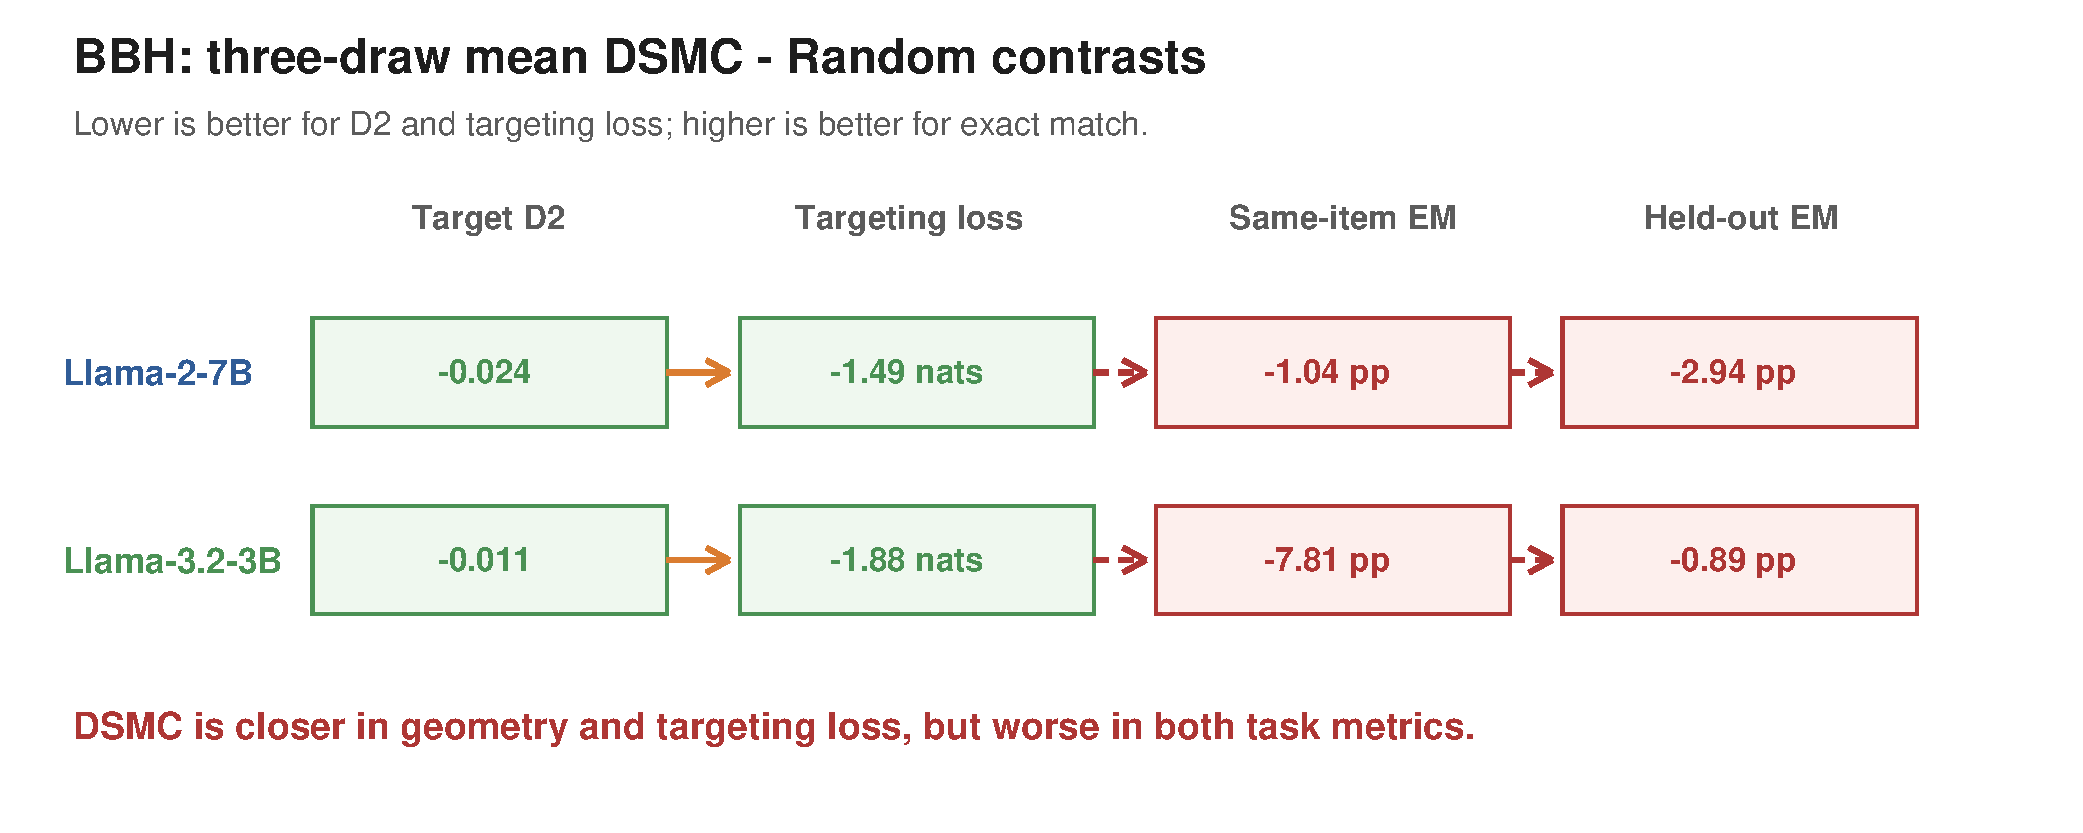
\includegraphics[width=\textwidth]{figures/surrogate_chain.pdf}
    \caption{\textbf{The proxy chain breaks on BBH in both model stacks.}
    \method{} has lower target discrepancy $\dsecond$ than Random, and the
    post-SFT teacher-forced loss underlying the targeting signal decreases,
    while same-item and held-out exact match fall. Every entry is the
    three-draw mean \method{}--Random contrast; lower values are favourable for
    $\dsecond$ and targeting loss but unfavourable for exact match. Arrows
    summarize measured relationships, not an identified causal mechanism.}
    \label{fig:chain}
\end{figure*}

\section{Target Matching with Directional Second Moments}
\label{sec:method}

\subsection{Targeted instruction selection}

Let $\mathcal{C}=\{x_i\}_{i=1}^{N}$ be a candidate instruction pool and
$\mathcal{Q}=\{q_j\}_{j=1}^{M}$ a small target query set. Given a budget $K$,
the goal is to select $\mathcal{S}\subset\mathcal{C}$, $|\mathcal{S}|=K$, such
that supervised fine-tuning on $\mathcal{S}$ improves held-out target
performance.

Following gradient-based targeted selection
\citep{xia2024less,nayak2026critical,mirzasoleiman2020craig,killamsetty2021gradmatch},
we compute per-example gradients at a
shared warm-up checkpoint and project them to a reusable low-dimensional
datastore. Following the optimizer-aware LESS protocol, candidates and queries
use role-specific transforms before entering a common projected directional
space:
\begin{equation}
    u_{\mathcal C}(x)
    =
    \frac{\Pi A_{\mathrm{Adam}}g(x)}
         {\|\Pi A_{\mathrm{Adam}}g(x)\|_2},
    \qquad
    u_{\mathcal Q}(q)
    =
    \frac{\Pi g(q)}
         {\|\Pi g(q)\|_2}.
    \label{eq:role_maps}
\end{equation}
Here $\Pi$ is a shared Rademacher projection and $A_{\mathrm{Adam}}$ denotes
the candidate-side optimizer-aware transform. The MMD identity below is exact
for these resulting unit vectors in the common projected space. The
construction should not, however, be interpreted as applying one symmetric
raw-gradient representation map to candidates and queries.

\subsection{Why a directional second moment?}

First-order mean-gradient matching represents a target by
$\mathbb{E}[u]$. This signed mean can cancel when useful examples occupy
opposite directions, even if they share the same underlying orientation.
We instead use the non-centered directional second moment
\begin{equation}
    M_P = \mathbb{E}_{u\sim P}[uu^\top].
    \label{eq:moment}
\end{equation}
Because $uu^\top=(-u)(-u)^\top$, this representation captures orientation
rather than sign. We deliberately call it a \emph{directional second moment},
not a covariance: the vectors are normalized and the mean is not subtracted.

Consider the positive semidefinite kernel
\begin{equation}
    k_2(u,v) = (u^\top v)^2.
\end{equation}
Since
$\langle uu^\top,vv^\top\rangle_F=(u^\top v)^2$, the biased empirical MMD
between a selected set $\mathcal{S}$ and query set $\mathcal{Q}$ is exactly
\citep{gretton2012mmd,muandet2017kme}
\begin{align}
    \operatorname{MMD}_{k_2}^2(\mathcal{S},\mathcal{Q})
    &=
    \left\|
    \frac{1}{|\mathcal{S}|}\sum_{s\in\mathcal{S}}u_su_s^\top
    -
    \frac{1}{|\mathcal{Q}|}\sum_{q\in\mathcal{Q}}u_qu_q^\top
    \right\|_F^2 \nonumber\\
    &\equiv \dsecond(\mathcal{S},\mathcal{Q}).
    \label{eq:mmd_identity}
\end{align}
The identity is algebraic: \method{} matches this empirical second moment
exactly as defined, but the kernel is not characteristic and does not identify
the full gradient distribution
\citep{sriperumbudur2011universality,muandet2017kme}.

\subsection{Exact greedy coreset construction}

For a candidate $x$, define target relevance and accumulated selected-set
similarity as
\begin{equation}
    r_{\mathcal Q}(x)=\frac{1}{|\mathcal Q|}
    \sum_{q\in\mathcal Q}k_2(u_x,u_q),
    \quad
    r_{\mathcal S}(x)=\sum_{s\in\mathcal S}k_2(u_x,u_s).
\end{equation}
At step $m=|\mathcal S|$, the exact one-step marginal for minimizing the biased
MMD selects
\begin{equation}
    x^\star =
    \arg\max_{x\notin\mathcal S}
    \left[
    r_{\mathcal Q}(x)
    -
    \frac{r_{\mathcal S}(x)+k_2(u_x,u_x)/2}{m+1}
    \right].
    \label{eq:greedy}
\end{equation}
For unit vectors $k_2(u_x,u_x)=1$. The first term rewards query alignment and
the second penalizes selected-set self-similarity. We use the deterministic
exact marginal throughout; we make no stochastic-greedy or submodularity
guarantee. The construction is related to kernel herding and greedy kernel-mean
approximation \citep{chen2010herding,bach2012herding}, but
Equation~\ref{eq:greedy} is the exact marginal of the finite-sample objective
used here.

\paragraph{Why proxy ordering need not survive training.}
For one small SGD step on the same query loss,
$L_Q(\theta-\eta g_S)-L_Q(\theta)\approx-\eta g_Q^\top g_S$ motivates
alignment locally. Our pipeline additionally applies role-specific transforms,
greedy construction, multi-step Adam in a LoRA subspace, generation, and exact
match. Equation~\ref{eq:ordering} would require this chain to preserve subset
order; our results do not contradict the local Taylor approximation.

\paragraph{Role in this paper.}
\method{} is a measurement instrument, not a claim of general selector
superiority. If it lowers $\dsecond$ relative to compared subsets without
improving utility, the reversal cannot be dismissed as failure to move its own
proxy.

\section{Experimental Design}
\label{sec:setup}

\subsection{Candidate pool, features, and training}

The candidate pool is the processed pool released with LESS
\citep{xia2024less}: 270,679 examples from Flan v2
\citep{longpre2023flan} (100,000), its CoT mixture (100,000), Dolly
\citep{dolly2023dataset} (15,011), and OASST1
\citep{kopf2024oasst1} (55,668). For each model stack, a LoRA
\citep{hu2022lora} warm-up checkpoint is used to construct a
candidate-gradient datastore. We use an
8,192-dimensional Rademacher projection with seed 123, unit-normalize the
projected vectors, and generate query-gradient caches separately for each draw.
The selected indices are materialized into static subsets; all downstream
comparisons restart from the corresponding base model rather than continuing
the warm-up run. We study Llama-2-7B and Llama-3.2-3B model stacks
\citep{touvron2023llama2,grattafiori2024llama3,meta2024llama32},
implemented through
LLaMA-Factory \citep{zheng2024llamafactory}.

Downstream SFT uses LoRA rank 128, alpha 512, dropout 0.05 on
\texttt{q/k/v/o\_proj}, learning rate $2\times10^{-5}$, linear decay, 3\%
warm-up, bfloat16, effective batch size 128, and four epochs. The 5\% budget is
$K=13{,}533$ (420 optimizer steps) and the 1\% budget is $K=2{,}707$ (84
steps). Full configurations, prompt templates, hashes, and data-processing
details are provided in Appendix~\ref{app:repro}.

\subsection{Target families}

\paragraph{MMLU controlled stress test.}
We construct ten globally disjoint 64-example query sets:
five STEM-majority draws (51 STEM, 13 humanities) and five
humanities-majority draws with the proportions reversed. Evaluation is balanced
accuracy
\[
\operatorname{BalAcc}
=\tfrac12(\operatorname{Acc}_{\mathrm{STEM}}
          +\operatorname{Acc}_{\mathrm{Humanities}})
\]
over held-out MMLU subjects \citep{hendrycks2021mmlu}. This is our
equal-category aggregate, not the benchmark's standard overall accuracy. Draw
index is paired with SFT seed
$\{42,1,2,3,4\}$; for comparisons shared across the two skew directions, the
primary descriptive unit is the five direction-averaged draw-index blocks.

\paragraph{BBH external validation.}
Using the BIG-Bench Hard suite \citep{suzgun2023bbh}, we construct within each
task family a disjoint query-reservoir/evaluation partition of the official
examples. The query reservoir contains 1,302 examples and the frozen held-out
partition contains 5,209. The evaluation harness exposes 27 subtasks spanning
23 conceptual BBH task families, because two families contain three
size-specific variants. Three stratified 64-example query draws define the
selection signals; we report the size-weighted micro exact-match aggregate over
the custom held-out partition using a pinned chain-of-thought few-shot
protocol. Each query/selection draw is crossed with two SFT seeds, which are
averaged \emph{within} the draw. The statistical unit is therefore the draw
($n=3$), not the six seed-level runs.

\subsection{Comparators and reporting policy}

The controlled gradient baselines are: first-order mean-gradient TopK
(LESS-style \citep{xia2024less}), first- and second-order relevance TopK,
first- and second-order round-robin (RR) \citep{nayak2026critical}, GIST
whitening on the shared projected datastore
(GIST-SharedProj \citep{min2026gist}), and a task-metric adaptation of NICE
(NICE-MMLU-EM \citep{wang2025nice}). Because several are shared-protocol adaptations rather than
full official end-to-end reproductions, we use these qualified names in the
paper. Target-independent controls are uniform Random-$K$, length-matched
Random on MMLU, a sequence/label-length-matched Random control on BBH, and a
shared no-SFT reference.

The study is descriptive. We report draw-level means, paired differences, and
win counts; we do not report significance tests over $n=3$ or $n=5$ blocks.
Subtask breakdowns and individual SFT seeds are diagnostics, not independent
replicates.

\section{Method Gains Are Stack-Dependent on MMLU}
\label{sec:mmlu}

\subsection{Llama-2 positive control}

\begin{table}[t]
\caption{\textbf{Llama-2 MMLU representation $\times$ selector attribution.}
Balanced accuracy at one fixed seed for each skew direction. In this stack,
the second-order representation improves both TopK and MMD; the smaller
DSMC--Second-TopK increment is within the measured training-noise scale and is
not treated as a stand-alone statistical claim.}
\label{tab:attribution}
\centering
\small
\begin{tabular}{lcccc}
\toprule
Target & 1st-TopK & 1st-MMD & 2nd-TopK & \method{} \\
\midrule
STEM-majority & 39.77 & 38.47 & 40.68 & \textbf{41.10} \\
Humanities-majority & 39.31 & 38.24 & 39.92 & \textbf{40.54} \\
\bottomrule
\end{tabular}
\end{table}

We first evaluate whether second-moment matching provides a meaningful
targeted-selection signal on MMLU.
Table~\ref{tab:attribution} factors the method into target
representation (signed first order versus directional second order) and
selection rule (relevance TopK versus MMD coreset). Moving to the second-order
representation improves both selectors in both skew directions:
$+0.61$--$0.91$ points under TopK and $+2.30$--$2.63$ points under MMD.
The selector interaction is representation dependent: first-order MMD hurts
relative to first-order TopK, while second-order MMD adds $0.42$--$0.62$
points over second-order TopK. The latter comparison is single-seed and small,
so this is a Llama-2 positive control, not a cross-stack method claim.

Across ten target draws at the 5\% budget,
\method{} beats LESS-style TopK and both RR baselines in every draw, and beats
the examined GIST and NICE adaptations in nine of ten draws
(Appendix~\ref{app:mmlu}). Relative to Second-RR, the mean gain is $0.88$
points and holds in all ten cells, supporting a complementary coreset effect at
this budget. The positive claim is deliberately scoped: in the studied
Llama-2 MMLU setting, directional second moments materially improve
target-aware selection.

The absolute comparison creates the first reversal. Against Random-$K$,
\method{} has a $-0.01$ point mean difference at 5\%, winning two of five
direction-averaged blocks; length-matched Random gives the same qualitative
conclusion. Tightening the budget does not rescue target awareness. At 1\%,
the \method{}--Random gap becomes $-0.77$ points and no query-direction cell
favours \method{}. The extra MMD gain over Second-RR also contracts to $0.17$
points and five of ten cells.

Most targeted methods fall below no-SFT at both budgets. However, the 1\% arm
is a positive-transfer ordering reversal in observed means: \method{} (40.17)
and Random (40.95) both exceed no-SFT (40.03), while \method{} is closer to
the leave-one-draw-out balanced target geometry in all ten draws. Thus the
ordering failure is not restricted to harmful SFT, although this deliberately
skewed stress test complements rather than replaces same-family BBH validation.
An equal-step sensitivity repeats the 1\% subsets to 420 steps; both \method{}
and Random fall to approximately 38.3\%, so extra optimization does not rescue
the targeted subset (Appendix~\ref{app:sensitivities}).

\subsection{Pre-specified cross-stack check}

\begin{table}[t]
\caption{\textbf{Cross-stack MMLU comparison at the 5\% budget.}
\method{}'s advantage over the two RR baselines is consistent on Llama-2-7B
but does not transfer to Llama-3.2-3B. \method{} and Random have nearly tied
observed means on both stacks. Win counts use the same five
direction-averaged draw-index blocks for both stacks; no significance test is
claimed.}
\label{tab:mmlu_crossstack}
\centering
\small
\begin{tabular}{lccc}
\toprule
Stack & \method{} $-$ First-RR & \method{} $-$ Second-RR
& \method{} $-$ Random \\
\midrule
Llama-2-7B & $+1.55$ (5/5) & $+0.88$ (5/5) & $-0.01$ (2/5) \\
Llama-3.2-3B & $-0.18$ (2/5) & $-0.31$ (1/5) & $+0.12$ (3/5) \\
\bottomrule
\end{tabular}
\end{table}

The cross-stack check does not support a transferable \method{} advantage.
Mean balanced accuracy is 47.95 for Second-RR, 47.82 for
First-RR, 47.64 for \method{}, and 47.52 for Random, while the no-SFT reference
is 49.47. All four methods lie within 0.44 points and below base.
Table~\ref{tab:mmlu_crossstack} shows the sharper contrast: \method{}'s
Llama-2 advantage over both RR arms reverses on Llama-3.2, whereas its
difference from Random remains close to zero on both stacks. Thus the
method-level advantage of \method{} does not transfer. In contrast, the BBH
geometry--utility counterexample below does.

\section{External Reversal on BBH}
\label{sec:bbh}

\begin{table*}[t]
\caption{\textbf{Held-out BBH exact match.} Means first average the two SFT
seeds within each of three query/selection draws. All method means are below
the corresponding no-SFT reference. \method{} loses to Random in every draw on
both model stacks, while achieving the lowest target second-moment discrepancy
among the compared subsets in every draw.}
\label{tab:bbh}
\centering
\small
\begin{tabular}{llrrrrr}
\toprule
Stack & Method & Draw 0 & Draw 1 & Draw 2 & Mean & $\Delta$ vs.\ no-SFT \\
\midrule
\multirow{5}{*}{Llama-2-7B}
& No-SFT & \multicolumn{4}{c}{39.64} & -- \\
& Random-$K$ & 39.30 & 38.78 & 39.67 & \textbf{39.25} & $-0.39$ \\
& First-RR & 36.24 & 37.61 & 37.61 & 37.15 & $-2.49$ \\
& Second-RR & 36.80 & 37.00 & 36.80 & 36.87 & $-2.77$ \\
& \method{} & 36.36 & 36.47 & 36.10 & 36.31 & $-3.33$ \\
\midrule
\multirow{5}{*}{Llama-3.2-3B}
& No-SFT & \multicolumn{4}{c}{47.11} & -- \\
& Random-$K$ & 47.32 & 46.61 & 47.17 & \textbf{47.03} & $-0.08$ \\
& First-RR & 46.11 & 46.52 & 47.04 & 46.56 & $-0.55$ \\
& Second-RR & 46.62 & 46.23 & 47.18 & 46.68 & $-0.44$ \\
& \method{} & 45.98 & 45.88 & 46.57 & 46.14 & $-0.97$ \\
\bottomrule
\end{tabular}
\end{table*}

MMLU queries are deliberately skewed, leaving open the possibility that the
selector faithfully follows an unrepresentative query sample. BBH removes this
specific explanation: queries and evaluation examples are held-out samples from
the same task family. In this setting, the geometry--utility reversal persists
(Table~\ref{tab:bbh}). On Llama-2-7B, Random reaches 39.25\% micro exact match,
while \method{} reaches 36.31\%, a $-2.94$ point paired gap with zero of three
draws favouring \method{}. Both RR variants also outperform \method{};
together with Table~\ref{tab:mmlu_crossstack}, this shows that a favourable
\method{} ranking is neither cross-task nor cross-stack.

The direction repeats on Llama-3.2-3B. Random remains best at 47.03\%, and
\method{} is last among the four shared arms at 46.14\%. The $-0.89$ point
gap is negative in all three draws. The magnitude is substantially attenuated:
all methods are within one point of the no-SFT model, so the two stacks should
not be presented as equally dramatic. They nevertheless agree on the direction
of the \method{}--Random gap.

\paragraph{All SFT means are below no-SFT.}
On Llama-2, Random is only $0.39$ points below the shared base reference, while
target-aware methods are $2.49$--$3.63$ points below it. On Llama-3.2, Random is
$0.08$ points below base and \method{} $0.97$ below. These are shared reference
lines rather than replicated treatments, so we describe the observed means
rather than claim inferentially established negative transfer. The SFT
infrastructure is not uniformly detrimental: under the same Llama-2 pipeline,
\method{} and Random are slightly above the no-SFT reference on MMLU at 5\%,
and Random is $0.92$ points above it at 1\%. We therefore treat BBH and
Llama-3.2 MMLU as observed negative-transfer regimes, not evidence that the
training implementation cannot produce gains.

\paragraph{Matched-format control.}
On Llama-2, constraining Random to match \method{}'s coarse sequence-length
$\times$ loss-bearing-label-length histogram lowers Random from 39.25\% to
38.05\%, but still leaves it 1.74 points above \method{}. This is consistent
with instruction-format or correlated provenance composition contributing to
the gap. It is not a causal decomposition: the control changes several
correlated properties simultaneously. Full results are in
Appendix~\ref{app:sensitivities}.

\section{Where the Surrogate Chain Breaks}
\label{sec:diagnostics}

\subsection{\method{} attains the lowest observed target discrepancy}

For every BBH draw, we compute the operational discrepancy used by \method{},
\begin{equation}
    \dsecond(\mathcal S,\mathcal Q_d)
    = \|M_{\mathcal S}-M_{\mathcal Q_d}\|_F^2.
\end{equation}
On Llama-2, mean $\dsecond$ is 0.0863 for \method{} and 0.1098 for Random;
on Llama-3.2 it is 0.0644 and 0.0752. More importantly, \method{} has the
lowest $\dsecond$ among the compared subsets in all three draws of both
stacks, while being worse than Random downstream in all three draws. This
direct 3/3-versus-3/3 counterexample is the primary geometry result;
descriptive rank correlations are reported only in
Appendix~\ref{app:geometry}.

This shows that the downstream reversal is not explained merely by \method{}
failing to reduce its intended discrepancy relative to the compared subsets;
it does not imply global optimality of the greedy solution. In MMLU, \method{}
is also closer than Random to a leave-one-draw-out balanced reference in all
ten draws at both budgets (Appendix~\ref{app:geometry}). Thus the observed
failure is not simply that \method{} follows a skewed query away from the
balanced reference.

\paragraph{Query-disjoint proxy geometry.}
We post-hoc score frozen subsets against 256 examples sampled after excluding
all selection queries, under a protocol frozen before proxy-gradient
extraction. Without reselection or SFT, \method{} remains closer than Random
under $\dsecond$, and First-RR under signed $D_1$, in all three draws on both
stacks; both remain worse downstream. The reversal therefore extends beyond
selection-example geometry (Appendix~\ref{app:proxy_geometry}).

\paragraph{Sign-sensitive first-moment diagnostic.}
The quadratic kernel is invariant to $u\mapsto -u$, so we also examine the
signed first-moment discrepancy
\begin{equation}
    D_1(\mathcal S,\mathcal Q)
    =
    \left\|
    \mathbb E_{\mathcal S}[u]-\mathbb E_{\mathcal Q}[u]
    \right\|_2 .
\end{equation}
First-RR is closer than Random under $D_1$ in all three draws on both stacks,
yet its held-out BBH mean is lower than Random by 2.10 points on Llama-2 and
0.48 points on Llama-3.2. The observed alignment--utility reversal is
therefore not confined to the sign-invariant second moment. This diagnostic
does not establish failure for every sign-sensitive representation; full
draw-level values are in Appendix~\ref{app:geometry}; the mean gaps
($0.471$ vs.\ $0.591$ and $0.459$ vs.\ $0.498$) are not epsilon effects.

\paragraph{Evaluation-matched target serialization.}
To test whether the \method{} minimum is induced by the chat serialization
used for target extraction, we re-extract only target gradients under the bare
evaluation serialization and rescore frozen subsets. Despite low cross-context
row cosine (0.25--0.36), \method{} retains the lowest $\dsecond$ in all draws
on both stacks while losing to Random downstream. The full Llama-3.2 ranking
changes in every draw, so we claim robustness only of the \method{}--Random
counterexample, not serialization-invariant rankings
(Appendix~\ref{app:evalctx}).

\subsection{The query loss underlying the targeting signal also improves}

Gradient-based targeting uses a differentiable final-answer objective to
construct query gradients. We therefore recompute teacher-forced final-answer
cross-entropy on the same query items, under the exact wrapped serialization
used by each stack's targeting pipeline. On Llama-2, all four target-aware
methods reduce this loss by 0.68--1.40 nats, while Random increases it by 0.33.
On Llama-3.2, the target-aware methods reduce it by 3.19--3.40 nats and Random
by only 1.37. The second stack therefore gives a magnitude split rather than a
sign split; on both stacks, the targeted methods produce larger reductions in
the query loss from which the targeting gradients are derived.

\subsection{Task utility does not follow on the same examples}

Comparing query loss to held-out exact match changes both metric and examples.
We consequently evaluate chain-of-thought exact match on the same 64 query
items. For Llama-2, every target-aware method's mean query exact match falls
relative to base ($-3.65$ to $-6.51$ points) despite the substantial
cross-entropy reductions. On Llama-3.2, all three targeted methods again have
negative mean changes, with \method{} falling by 6.51 points; Random changes by
$+1.30$ points. The individual 64-item draw metrics are coarse---one item is
1.56 points---but the mean separation is consistent with the held-out ranking.

The same-item analysis rules out a purely query-to-test generalization account:
the downstream metric does not improve even on the examples that form the
targeting signal. It does not rule out every form of overfitting, nor does it
identify the missing mechanism.

\paragraph{Task-level breadth.}
The draw remains the primary experimental unit. A secondary 27-subtask
breakdown shows that \method{} trails Random on 23 subtasks and leads on four
for Llama-2 (macro difference $-2.89$ points). On Llama-3.2 it trails on 17
and leads on ten (macro difference $-1.10$). A descriptive bootstrap over
subtasks gives intervals of $[-4.68,-1.41]$ and $[-2.57,+0.27]$ points,
respectively. Thus the Llama-2 gap is broad across subtasks, whereas the
smaller Llama-3.2 effect is more heterogeneous. Regrouping size variants into
the 23 conceptual BBH families gives the same reading: 20/23 and 14/23
families favour Random.

\paragraph{Parser-validity audit.}
A post-hoc audit of all frozen generations finds invalid-rate contrasts of
$+0.03$ points on Llama-2 and $-0.78$ on Llama-3.2. \method{} remains below
Random conditional on standard-valid outputs ($-3.13$, $-1.36$ points) and
under frozen conservative recovery ($-3.08$, $-0.84$), so parsing does not
explain the gap (Appendix~\ref{app:parser}).

\subsection{Serialization narrows the loss-based diagnostic}

The targeting loss uses each stack's LLaMA-Factory wrapper
\citep{zheng2024llamafactory}, whereas BBH generation uses a pinned bare
evaluation context implemented through the language-model evaluation harness
\citep{biderman2024evaluation}. Recomputing final-answer
cross-entropy on that bare context yields different behavior across stacks. On
Llama-2, no method improves bare-context CE, although targeted methods degrade
it much less than Random. On Llama-3.2, target-aware methods do improve
bare-context CE while Random does not. Therefore we do \emph{not} claim that
final-answer cross-entropy is inherently misaligned with chain-of-thought
generation. The supported claim is narrower: the targeting loss used to
construct query gradients can decrease on the defining examples without a
corresponding improvement in chain-of-thought exact match, and this relationship
is serialization- and model-stack-dependent.

\section{Related Work}
\label{sec:related}

\paragraph{Instruction data selection.}
General-purpose instruction selection commonly scores data for quality,
difficulty, and diversity. DEITA jointly studies complexity, quality, and
diversity for data-efficient alignment \citep{liu2024deita}. Get More for Less
studies selection for the warm-up stage before target fine-tuning
\citep{kang2024getmore}. TSDS uses a small target set to define an
optimal-transport distribution-alignment objective
\citep{liu2024tsds}. Our focus is on testing whether attaining a better
query-derived proxy value is sufficient for utility.

\paragraph{Distribution matching and gradient coresets.}
MMD and kernel mean embeddings define set-level distribution discrepancies
\citep{gretton2012mmd,muandet2017kme}; characteristic-kernel results specify
when these discrepancies identify distributions
\citep{sriperumbudur2011universality}. Kernel herding greedily approximates a
target kernel mean \citep{chen2010herding,bach2012herding}, while CRAIG and
GRAD-MATCH use gradient geometry for data-efficient training
\citep{mirzasoleiman2020craig,killamsetty2021gradmatch}. Our novelty is not
the quadratic-kernel identity or greedy moment matching in isolation, but their
use as a directly measurable intervention for testing whether stronger
target-gradient alignment is sufficient for downstream utility.

\paragraph{Targeted and influence-based selection.}
LESS builds reusable low-dimensional gradient datastores and uses
optimizer-aware gradient similarity for targeted instruction tuning
\citep{xia2024less}. NICE replaces next-token-loss influence with a
policy-gradient construction tied to non-differentiable evaluation metrics
\citep{wang2025nice}. GIST recovers a target-gradient subspace and scores
candidate alignment under coupled optimization geometry
\citep{min2026gist}. GIO uses examples representing a target distribution to
optimize a scalable gradient-information objective for dataset selection
\citep{everaert2024gio}. A recent controlled study separates representations
from selection algorithms and finds that gradient representations are often
predictive, but no single selector dominates across settings
\citep{nayak2026critical}. Where that study asks which representations and
selectors are predictive across settings, we ask whether attaining a better
value of a measurable target geometry is itself sufficient for greater
downstream utility.

\paragraph{Surrogate mismatch and strong Random baselines.}
ROSE motivates reward-oriented selection by documenting non-monotonicity
between instruction-tuning loss and task reward \citep{wu2025rose}; NICE makes
a related move from differentiable training loss to task metrics
\citep{wang2025nice}. Controlled studies also find that sophisticated
selectors may fail to consistently outperform Random
\citep{diddee2025chasing,xia2025random}. Together, our diagnostics establish an empirical
counterexample in which lower target discrepancy and lower targeting loss do
not yield higher task utility.

\section{Limitations}
\label{sec:limitations}

The study covers two model stacks, one candidate pool, and two target families;
a stack changes model, tokenizer, and serialization together. BBH has only
three query/selection draws and the 3B effect is small. On Llama-3.2 MMLU, all
methods are within 0.44 points and below no-SFT. MMLU also couples draw index
to SFT seed, so five direction-averaged blocks, not ten cells, carry shared
comparisons.

Candidates use Adam-aware features whereas queries use raw SGD gradients, so
claims concern this operational push-forward geometry rather than symmetric
raw-gradient matching. Evaluation-matched rescoring does not remove this
asymmetry, and the finer Llama-3.2 ranking changes in every draw.

Several baselines are controlled adaptations rather than full end-to-end
reproductions. Contamination checks are lexical, not semantic. The diagnostics
do not identify a unique causal mechanism: format and provenance remain
plausible, the query-disjoint proxy only rescores frozen subsets from the query
reservoir, and the parser audit tests extraction rather than semantic
correctness.

\section{Conclusion}

What transfers across the two tested model stacks is not \method{}'s method
advantage, but a counterexample to the sufficiency of the studied selection
objective.
Across the positive-transfer MMLU 1\% comparison and the negative-transfer BBH
regime, lower values of the studied operational first- and second-moment
gradient discrepancies do not guarantee higher downstream utility. A better
value of a query-derived selection objective should therefore be treated as
progress only after its relationship to the downstream task metric has been
independently validated.

\subsection*{AI use statement}

Generative AI tools were used to summarize and cross-check existing literature,
inspect repository artifacts, suggest paper structure and wording, draft and
edit parts of the manuscript, and assist with software implementation and
analysis scripts. Earlier in the research workflow, generative AI tools also
provided feedback on experimental design and result interpretation. The
authors reviewed all AI-assisted text, code, and claims against the underlying
implementations, configurations, manifests, and result files; all reported
numerical results were computed from experiment artifacts rather than
generated by an AI system. The authors take responsibility for the final
content, including all AI-assisted material.

\subsection*{Ethics statement}

This work studies data selection for publicly available language-model
benchmarks and does not involve human-subject data collection. The main risks
are those shared by instruction tuning, including inherited dataset biases,
benchmark contamination, and overgeneralization from a limited experimental
scope. We report negative results, adapted-baseline scope, and contamination
audit limits explicitly to reduce the risk of overstating practical
conclusions.

\subsection*{Reproducibility statement}

Appendix~\ref{app:repro} documents the data composition, target-draw
construction, feature protocol, selection rules, training hyperparameters,
evaluation pins, statistical units, and integrity checks. The supplementary
material will include anonymized code, exact run configurations, frozen
manifests and hashes, paper tables generated from committed result files, and
the timestamped, pre-outcome protocol specifications for the BBH and
second-model experiments.

\bibliography{references}
\bibliographystyle{iclr2027_conference}

\appendix

\section{Method Derivations}
\label{app:derivations}

\subsection{MMD identity}

Let
$\widehat M_{\mathcal S}=|\mathcal S|^{-1}\sum_{s\in\mathcal S}u_su_s^\top$
and define $\widehat M_{\mathcal Q}$ analogously. Expanding the squared
Frobenius norm gives
\begin{align}
\|\widehat M_{\mathcal S}-\widehat M_{\mathcal Q}\|_F^2
&=
\frac{1}{|\mathcal S|^2}\sum_{s,s'}
\langle u_su_s^\top,u_{s'}u_{s'}^\top\rangle_F \nonumber\\
&\quad+
\frac{1}{|\mathcal Q|^2}\sum_{q,q'}
\langle u_qu_q^\top,u_{q'}u_{q'}^\top\rangle_F \nonumber\\
&\quad-
\frac{2}{|\mathcal S||\mathcal Q|}\sum_{s,q}
\langle u_su_s^\top,u_qu_q^\top\rangle_F \\
&=
\frac{1}{|\mathcal S|^2}\sum_{s,s'}(u_s^\top u_{s'})^2
+\frac{1}{|\mathcal Q|^2}\sum_{q,q'}(u_q^\top u_{q'})^2
-\frac{2}{|\mathcal S||\mathcal Q|}\sum_{s,q}(u_s^\top u_q)^2.
\end{align}
This is the biased empirical MMD under $k_2$.

\subsection{Greedy marginal}

Terms depending only on $\mathcal Q$ can be dropped. Comparing the objective
after adding $x$ to a set of size $m$ yields Equation~\ref{eq:greedy} after
positive rescaling. The implementation maintains $r_{\mathcal S}(x)$
incrementally and masks selected or invalid rows. Zero and non-finite feature
rows are rejected before selection.

\section{Additional MMLU Results}
\label{app:mmlu}

\begin{table}[h]
\caption{\textbf{Llama-2 MMLU target-draw results.} Mean equal-domain balanced
accuracy over ten query draws (five paired draw-index blocks). The no-SFT
reference is shared, not a replicate.}
\label{tab:mmlu_main}
\centering
\small
\begin{tabular}{lcc}
\toprule
Method & 5\% & 1\% \\
\midrule
No-SFT & 40.03 & 40.03 \\
LESS-style TopK & 39.41 & 39.37 \\
First-RR & 38.80 & 38.20 \\
Second-RR & 39.48 & 40.00 \\
GIST-SharedProj & 38.85 & 39.45 \\
NICE-MMLU-EM & 39.25 & 39.42 \\
\method{} & 40.36 & 40.17 \\
Random-$K$ & 40.37 & \textbf{40.95} \\
Length-matched Random & \textbf{40.42} & 40.80 \\
\bottomrule
\end{tabular}
\end{table}

\paragraph{Pre-specified Llama-3.2 outcome.}
The 5\% cross-stack arm completed 35/35 adapters and 36/36 evaluations with no
failures. The statistical unit is five direction-averaged draw-index blocks.
The protocol was committed before the second-model computations. The no-SFT
balanced reference is 49.47; mean balanced accuracy is 47.95 for
Second-RR, 47.82 for First-RR, 47.64 for \method{}, and 47.52 for Random.
\method{} minus First-RR is $-0.18$ points (2/5 blocks), minus Second-RR is
$-0.31$ (1/5), and minus Random is $+0.12$ (3/5). This is the
pre-specified outcome in which the Llama-2 method advantage does not transfer.

\paragraph{Lower budget and equal-step sensitivity.}
On Llama-2, \method{} minus Random changes from $-0.01$ points at 5\% to
$-0.77$ at 1\%, with 0/10 1\% cells favouring \method{}. Repeating the 1\%
\method{} and Random subsets to the 420 steps used by the 5\% arm reduces both
to approximately 38.3\%, about 1.8 points below the shared no-SFT reference.
Thus the low-budget comparison is not rescued by simply increasing optimizer
steps.

\section{Additional Geometry Diagnostics}
\label{app:geometry}

On MMLU, a leave-one-draw-out balanced reference gives mean $\dsecond$ values
of 0.1538 for \method{} and 0.1762 for Random at 5\%, and 0.1522 versus
0.1764 at 1\%; \method{} is closer in all ten draws at each budget. On BBH,
the descriptive Spearman correlation between $\dsecond$ and accuracy is
positive in all three Llama-2 draws (0.77, 0.83, 0.89 over six methods) and all
three Llama-3.2 draws (0.80, 1.00, 0.20 over four methods). These ranking
samples are small and no inferential interpretation is attached to them.

\begin{table}[h]
\caption{\textbf{Signed first-moment discrepancy on BBH.}
$D_1=\|\mathbb E_{\mathcal S}[u]-\mathbb E_{\mathcal Q}[u]\|_2$ is
sign-sensitive. First-RR is closer than Random in every draw, yet its
downstream mean is lower on both stacks.}
\label{tab:signed_d1}
\centering
\small
\begin{tabular}{llrrr}
\toprule
Stack & Draw & \method{} & First-RR & Random \\
\midrule
Llama-2 & 0 & 0.4886 & \textbf{0.4763} & 0.5957 \\
        & 1 & 0.4972 & \textbf{0.4861} & 0.6032 \\
        & 2 & 0.4610 & \textbf{0.4516} & 0.5741 \\
\midrule
Llama-3.2 & 0 & \textbf{0.4404} & 0.4611 & 0.5012 \\
          & 1 & \textbf{0.4599} & 0.4789 & 0.5179 \\
          & 2 & \textbf{0.4081} & 0.4374 & 0.4736 \\
\bottomrule
\end{tabular}
\end{table}

\begin{table}[h]
\caption{\textbf{Task-level DSMC--Random heterogeneity.}
Win/tie/loss counts and macro statistics average SFT seeds and query draws
within each of the 27 harness subtasks. Bootstrap intervals resample subtasks
and are descriptive; they do not replace the pre-specified draw-level unit.}
\label{tab:taskwise}
\centering
\small
\begin{tabular}{lrrrr}
\toprule
Stack & W/T/L & Macro $\Delta$ & Median $\Delta$ & Task-bootstrap 95\% \\
\midrule
Llama-2 & 4/0/23 & $-2.89$ & $-1.67$ & $[-4.68,-1.41]$ \\
Llama-3.2 & 10/0/17 & $-1.10$ & $-0.92$ & $[-2.57,+0.27]$ \\
\bottomrule
\end{tabular}
\end{table}

When the size-specific logical-deduction and shuffled-object subtasks are
regrouped into the 23 conceptual BBH families, \method{} wins/ties/loses
3/0/20 families on Llama-2 and 9/0/14 on Llama-3.2. Family-macro differences
are $-2.94$ and $-1.23$ points, with descriptive task-family bootstrap
intervals $[-4.94,-1.25]$ and $[-2.91,+0.26]$.

\section{Query-Disjoint Proxy Geometry}
\label{app:proxy_geometry}

This post-hoc target-only analysis follows a protocol frozen before the proxy
gradients were extracted. Starting from the 1,302-example BBH query reservoir,
we exclude the 185 distinct examples appearing in any selection query and
sample 256 examples by deterministic proportional stratification over the 27
harness subtasks (seed 20260827). The resulting proxy set is disjoint from
every selection query. We rescore only the frozen subsets; no selection,
training, or downstream evaluation is rerun.

\begin{table}[h]
\caption{\textbf{Geometry against the query-disjoint BBH proxy set.}
Lower is better. The frozen \method{} subset is closer than Random under
$D_2$ in every stack--draw cell; First-RR is closer than Random under signed
$D_1$ in every cell.}
\label{tab:proxy_geometry}
\centering
\small
\begin{tabular}{lllrrrr}
\toprule
Stack & Draw & Metric & \method{} & First-RR & Second-RR & Random \\
\midrule
Llama-2 & 0 & $D_1$ & 0.46684 & \textbf{0.45508} & 0.50589 & 0.57679 \\
        &   & $D_2$ & \textbf{0.07067} & 0.07250 & 0.07482 & 0.09445 \\
        & 1 & $D_1$ & 0.46540 & \textbf{0.45579} & 0.50108 & 0.57522 \\
        &   & $D_2$ & \textbf{0.07069} & 0.07256 & 0.07409 & 0.09360 \\
        & 2 & $D_1$ & 0.46524 & \textbf{0.45562} & 0.50093 & 0.57786 \\
        &   & $D_2$ & \textbf{0.07067} & 0.07237 & 0.07392 & 0.09412 \\
\midrule
Llama-3.2 & 0 & $D_1$ & \textbf{0.41998} & 0.44544 & 0.43849 & 0.48214 \\
          &   & $D_2$ & \textbf{0.05035} & 0.06087 & 0.05868 & 0.06056 \\
          & 1 & $D_1$ & \textbf{0.42084} & 0.44568 & 0.43871 & 0.48190 \\
          &   & $D_2$ & \textbf{0.05037} & 0.06083 & 0.05886 & 0.06132 \\
          & 2 & $D_1$ & \textbf{0.41935} & 0.44450 & 0.44258 & 0.48403 \\
          &   & $D_2$ & \textbf{0.05034} & 0.06230 & 0.06010 & 0.06103 \\
\bottomrule
\end{tabular}
\end{table}

The proxy comes from the held-out query reservoir, not the 5,209-example
downstream evaluation partition. These results establish frozen-subset
geometry ordering only and do not show what would happen after selecting and
training directly against the proxy target.

\section{Evaluation-Matched Target-Geometry Sensitivity}
\label{app:evalctx}

This post-hoc check changes only target serialization; it does not rerun
selection or SFT. Mean row cosine between operational and evaluation-matched
target gradients is 0.335/0.342/0.363 for Llama-2 and
0.249/0.270/0.272 for Llama-3.2.

\begin{table}[h]
\caption{\textbf{Evaluation-matched $\dsecond$ for frozen BBH subsets.}
Lower is better. The frozen \method{} subset is closest in all six
stack--draw cells, but the non-\method{} ranking changes in all three
Llama-3.2 draws.}
\label{tab:evalctx}
\centering
\small
\begin{tabular}{llrrrr}
\toprule
Stack & Draw & \method{} & First-RR & Second-RR & Random \\
\midrule
Llama-2 & 0 & \textbf{0.06675} & 0.06830 & 0.07102 & 0.08875 \\
        & 1 & \textbf{0.08230} & 0.08393 & 0.08586 & 0.10358 \\
        & 2 & \textbf{0.05655} & 0.05800 & 0.05989 & 0.07831 \\
\midrule
Llama-3.2 & 0 & \textbf{0.07985} & 0.09134 & 0.08921 & 0.08847 \\
          & 1 & \textbf{0.07660} & 0.08809 & 0.08619 & 0.08598 \\
          & 2 & \textbf{0.07124} & 0.08414 & 0.08203 & 0.08051 \\
\bottomrule
\end{tabular}
\end{table}

\section{Sensitivity and Falsification Checks}
\label{app:sensitivities}

\paragraph{Matched Random controls.}
MMLU length-matched Random gives the same qualitative target-awareness result
as plain Random. On Llama-2 BBH, sequence$\times$label-length-matched Random
scores 38.05, between plain Random (39.25) and \method{} (36.31). The control
changes correlated provenance and content as well as format, so it does not
support a causal percentage decomposition.

\paragraph{Same-item and bare-context diagnostics.}
On Llama-2, targeted methods reduce the wrapped targeting loss by
0.68--1.40 nats but their same-item CoT exact match changes by
$-3.65$ to $-6.51$ points. Under the bare evaluation context, no method
improves CE; targeted methods degrade it less than Random. On Llama-3.2,
targeted methods reduce wrapped targeting loss by 3.19--3.40 nats and also
reduce bare CE
by 0.41--0.57, while their mean same-item CoT changes remain negative. This is
why the loss-based diagnostic is tied to the tested targeting pipeline, not
cross-entropy in general.

\paragraph{Task exposure.}
Per-task query frequency has negative descriptive correlations with
targeted-vs-Random subtask deltas ($-0.210$, $-0.280$, $-0.224$ across the
three draws). We find no evidence for a simple account in which greater query
exposure protects a BBH task. This diagnostic is exploratory and does not
identify an alternative mechanism.

\section{Parser-Validity Audit}
\label{app:parser}

We audit every saved BBH generation without regenerating outputs. Conditional
EM is computed only over examples accepted by the standard harness parser.
For standard-invalid outputs, a frozen conservative rule inspects only the
final 500 characters and extracts a type-constrained final candidate: the last
parenthesized option, boolean/yes--no token, or standalone number when
applicable, otherwise the last explicit answer marker or nonempty line.
Unrecovered outputs remain incorrect. This secondary rule is not a replacement
for the primary metric.

\begin{table}[h]
\caption{\textbf{BBH parser-validity audit.}
Rates first average the two SFT seeds within each draw and then the three
draws. Conservative EM applies the frozen recovery rule only to
standard-invalid outputs.}
\label{tab:parser}
\centering
\small
\begin{tabular}{llrrr}
\toprule
Stack & Method & Standard valid & Conditional EM & Conservative EM \\
\midrule
Llama-2 & \method{} & 93.46 & 38.85 & 36.42 \\
        & Random & 93.50 & 41.98 & 39.50 \\
Llama-3.2 & \method{} & 94.42 & 48.87 & 46.77 \\
          & Random & 93.64 & 50.23 & 47.61 \\
\bottomrule
\end{tabular}
\end{table}

The \method{}--Random invalid-rate difference is $+0.03$ percentage points on
Llama-2 and $-0.78$ on Llama-3.2. The corresponding conditional-EM
differences are $-3.13$ and $-1.36$ points, and conservative-EM differences
are $-3.08$ and $-0.84$. Thus the observed utility ordering is not produced
merely by more \method{} outputs failing the standard parser. The audit does
not establish semantic correctness beyond these extraction rules.

\section{Baseline Implementations}
\label{app:baselines}

LESS-style TopK uses one shared checkpoint and mean signed gradient similarity;
it is not the official multi-checkpoint LESS pipeline. GIST-SharedProj applies
the paper's target-subspace whitening construction to the experiment's shared
normalized projected caches. NICE-MMLU-EM uses eight Monte Carlo samples and
an exact-match task reward in the common feature protocol. These adaptations
are intended to isolate representation and selection effects under controlled
features; the paper does not claim exact end-to-end reproduction of the
official systems.

\section{Contamination and Prompt Audits}
\label{app:audits}

Against MMLU and held-out BBH, normalized exact matching finds zero candidate
duplicates. Full-pool fuzzy screening finds zero pairs above Jaccard 0.3;
seven MMLU and five BBH 13-gram hits were manually reviewed and judged
boilerplate false positives. The BBH few-shot audit finds no exact duplicates
and is recorded as pass-with-disclosure for fuzzy near-duplicates. Prompt
parity, few-shot leakage, and token-truncation audits are included in the
supplementary artifact. A semantic embedding nearest-neighbor contamination
audit was \emph{not} performed, so these checks are lexical screens rather
than a complete decontamination certificate.

\section{Reproducibility Details}
\label{app:repro}

The candidate pool contains 270,679 examples. Projected gradients use dimension
8,192 and seed 123. MMLU target draws are globally disjoint; BBH uses three
stratified 64-example query draws and a 5,209-example held-out set. Frozen
manifests record target files, gradient tensors, selections, materialized
subsets, adapters, and evaluation-result hashes. All BBH evaluations pass
27-subtask/5,209-example gates, and all Llama-3.2 MMLU evaluations pass
57-subject gates. Selection-level stability was checked after target-gradient
non-bit-reproducibility was observed; the worst selector changed 5 of 2,707
indices. A paper-level artifact manifest maps each major figure and table to
its committed result files, analysis code, and frozen protocol.

\subsection{Compute and selection overhead}

\begin{table}[h]
\caption{\textbf{Representative measured or launch-accounted costs on eight
NVIDIA H20 GPUs.} Candidate datastores are reusable across target draws and
tasks for a fixed model stack. Times for target gradients and selectors are
coarse stage-level accounting rather than microbenchmarks.}
\label{tab:cost}
\centering
\small
\begin{tabular}{lll}
\toprule
Stage & Reuse scope & Representative cost \\
\midrule
Warm-up checkpoint & per model stack & $\sim$1.5 GPU-h \\
Candidate gradient datastore & across targets & $\sim$6--8 GPU-h per stack \\
Three BBH target caches & per query draws & $\sim$1 GPU-h \\
\method{} + First/Second-RR & per three draws & $\sim$1.5 GPU-h \\
Random-$K$ sampling & per subset & negligible \\
Llama-3.2 BBH SFT, 24 adapters & per selected subsets & 3.39 GPU-h measured \\
Llama-3.2 MMLU SFT, 35 adapters & per selected subsets & 16.88 GPU-h measured \\
Llama-2 BBH SFT, 36 adapters & per selected subsets & 13.18 GPU-h measured \\
\bottomrule
\end{tabular}
\end{table}

The main practical asymmetry is therefore not the greedy selector alone but the
model-in-the-loop feature pipeline: Random requires neither warm-up nor
gradient datastores. The anonymous supplement will include sanitized
configurations and manifests. Before release, absolute cluster paths, Git
metadata, user names, and repository links must be removed.

\end{document}
